\par\medskip
\noindent\begin{minipage}{\columnwidth}
  \centering
  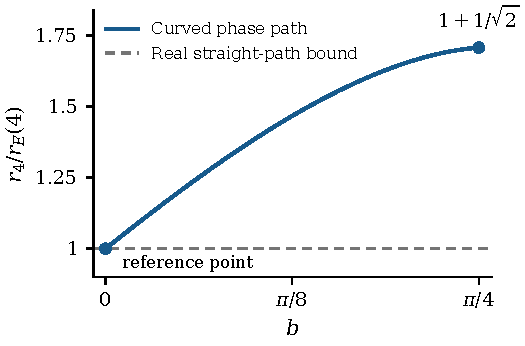
\includegraphics[width=\columnwidth]{figures/fig3_curved.pdf}
  \captionof{figure}{Radius increase at $n=4$ along the explicit curved phase path.
  The solid curve is $r_4/r_E(4)=\cos[b+\delta(b)]-\sin\delta(b)$, evaluated using the closed-form root $\delta(b)$ in Eq.~\eqref{low:delta} on $0\leq b\leq\pi/4$; the reference radius is $r_E(4)=\sqrt3/8$.
  It increases strictly from $1$ to $1+1/\sqrt2$.
  The dashed level is the radius bound for all admissible real straight phase paths through the specified reference point.}
  \label{fig:curved}
\end{minipage}
\par\medskip
